\chapter{Conclusão}\label{sec:conclusion}

De uma forma geral, o progresso do projeto está de acordo com o planeamento apresentado anteriormente, na proposta de projeto, e novamente, na figura~\ref{fig:timeline}.

Inicialmente, devido à pesquisa e aprendizagem de algumas tecnologias novas, o desenvolvimento ocorreu de forma mais lenta. 
No entanto, após ultrapassado esse obstáculo, o ritmo de trabalho aumentou de forma considerável e consequentemente os resultados surgiram também mais rapidamente. 

De momento, a aplicação já possui um modelo de dados estruturado e algumas funcionalidades, nomeadamente a possibilidade de criação, 
inscrição e visualização de uma necessidade, e um \textit{back office} que permite adicionar e/ou remover categorias possíveis de uma necessidade. 
Para além disto, foi desenvolvida uma outra funcionalidade que estava no planeamento ser realizada no próximo sprint, nomeadamente a visualização das necessidades dispostas num calendário.

\begin{figure}[H]
  \centering 
  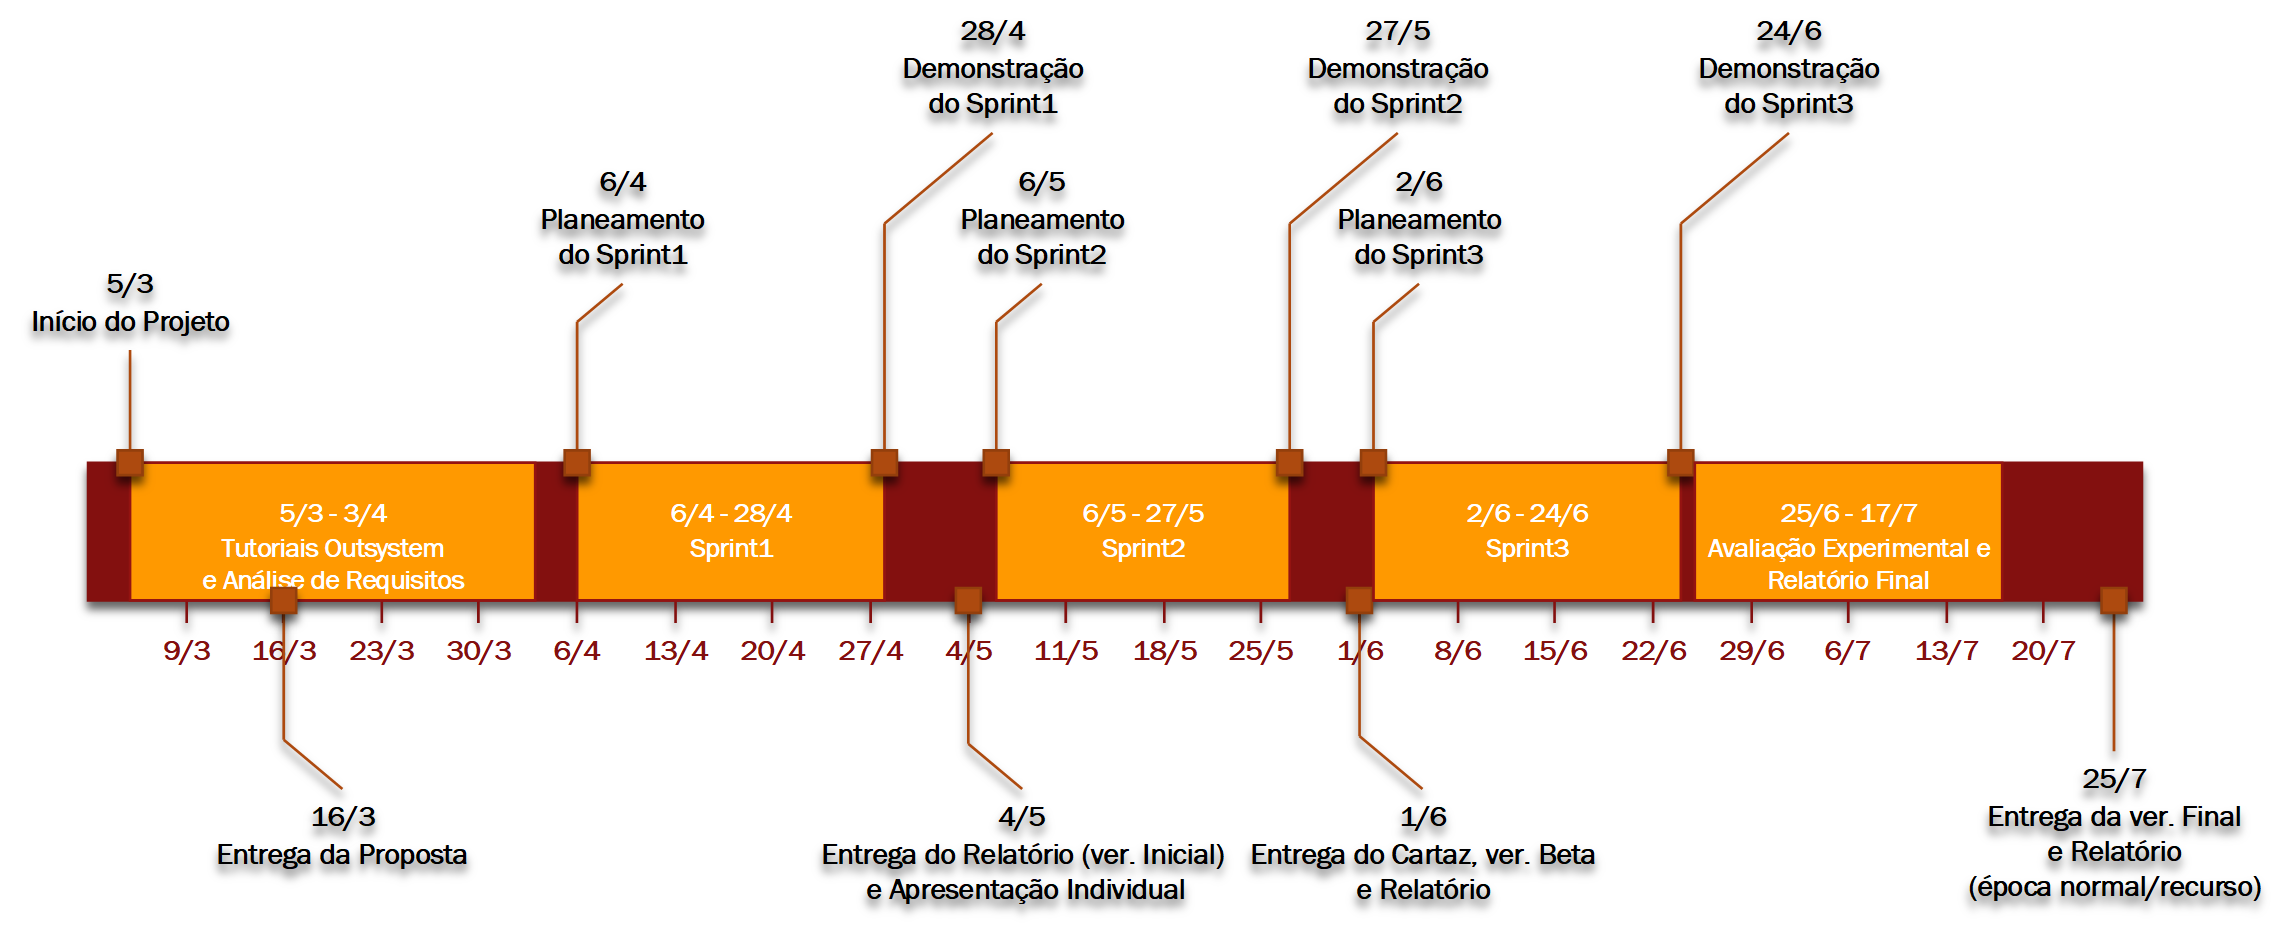
\includegraphics[scale=0.5]{figures/Timeline.png}
  \caption{Timeline}\label{fig:timeline}
\end{figure}